% vim: set textwidth=78 autoindent:
% !TeX  root  =  user_guide.tex 

\section{GDAL Werkzeuge}\label{label_plugingdaltools}

% when the revision of a chapter has been finalized, 
% comment out the following line:
% \updatedisclaimer

\subsection{Was sind die GDAL Werkzeuge?}\label{whatsgdal}

Die GDAL Werkzeuge stellen eine grafische Benutzeroberfl�che bereit, �ber die die 
verschiedenen Werkzeuge der Geospatial Data Abstraction Library (GDAL), 
\url{http://gdal.osgeo.org} angesprochen werden k�nnen. Dabei handelt es sich um Raster 
Management Tools, z.B. f�r die Abfrage, Umprojizierung, Transformierung oder Verschneidung 
von Rasterlayern in unterschiedlichen Formaten. Au�erdem stehen Werkzeuge zur Verf�gung, 
um Konturen als Vektorlinien zu extrahieren, eine Schummerungskarte aus H�hendaten zu 
erzeugen oder ein VRT (Virtual Raster Tile in XML format) aus einer oder mehrerer 
Rasterkarten zu erzeugen. Diese Werkzeuge k�nnen benutzt werden, wenn installiert und 
aktiviert wurde. 

\subsection{Die GDAL Bibliothek}\label{gdal_lib}

Die GDAL Bibliothek besteht aus einer Reihe von Kommandozeilen-Tools, jedes mit zahlreichen 
Optionen. Anwender, die sich mit der Kommandozeile auskennen, werden diese Art der Anwendung 
sicher bevorzugen, um so den vollen Funktionsumfang nutzen zu k�nnen. Das GDAL Tools Plugin 
erm�glicht hingegen einen einfachen Zugang zu den Funktionen, und stellt daher auch nur die 
am h�ufigsten benutzten Optionen zur Verf�gung.   

\begin{longtable}{|p{3cm}|p{13cm}|}
\caption{Liste der GDAL Werkzeuge}\label{tab:gdaltools} \\
\hline
Virtuelle(n) Raster(Katalog) erzeugen & Dieses Werkzeug erstellt ein VRT (Virtuellen Datensatz), 
das ein Mosaik der Eingaberaster darstellt. \\
\hline Kontur & Dieses Werkzeug erstellt einen Vektorlayer mit den Konturlinien eines 
H�hemnmodells (DGM).\\
\hline Rastern &  Dieses Werkzeug This program burns vector geometries (points, lines and polygons) into the raster band(s) of a raster image. Vectors are read from OGR supported vector formats. Note that the vector data must in the same coordinate system as the raster data; on the fly reprojection is not provided.\\
\hline Polygonisieren & This utility creates vector polygons for all connected regions of pixels in the raster sharing a common pixel value. Each polygon is created with an attribute indicating the pixel value of that polygon. A raster mask may also be provided to determine which pixels are eligible for processing.
The utility will create the output vector datasource if it does not already exist, defaulting to GML format.\\
\hline Verschmelzen &  This utility will automatically mosaic a set of images. All the images must be in the same coordinate system and have a matching number of bands, but they may be overlapping, and at different resolutions. In areas of overlap, the last image will be copied over earlier ones. \\
\hline Sieben & The gdal\_sieve.py script removes raster polygons smaller than a provided threshold size (in pixels) and replaces replaces them with the pixel value of the largest neighbour polygon. The result can be written back to the existing raster band, or copied into a new file.\\
\hline Nachbarschaft & The gdal\_proximity.py script generates a raster proximity map indicating the distance from the center of each pixel to the center of the nearest pixel identified as a target pixel. Target pixels are those in the source raster for which the raster pixel value is in the set of target pixel values.\\
\hline Fast schwarz & This utility will scan an image and try to set all pixels that are nearly black (or nearly white) around the collar to exactly black (or white). This is often used to "fix up" lossy compressed airphotos so that color pixels can be treated as transparent when mosaicing.\\
\hline Entzerren & The gdalwarp utility is an image mosaicing, reprojection and warping utility. The program can reproject to any supported projection, and can also apply GCPs stored with the image if the image is 'raw' with control information. \\
\hline Gitter & This program creates regular grid (raster) from the scattered data read from the OGR datasource. Input data will be interpolated to fill grid nodes with values, you can choose from various interpolation methods.\\
\hline Konvertieren & The gdal\_translate utility can be used to convert raster data between different formats, potentially performing some operations like subsettings, resampling, and rescaling pixels in the process.\\
\hline Information & The gdalinfo program lists various information about a GDAL supported raster dataset. \\
\hline Projektion zuweisen &  The gdalwarp utility is an image mosaicing, reprojection and warping utility. The program can reproject to any supported projection, and can also apply GCPs stored with the image if the image is 'raw' with control information.
-s\_srs srs def:
source spatial reference set. The coordinate systems that can be passed are anything supported by the OGRSpatialReference.SetFromUserInput() call, which includes EPSG PCS and GCSes (ie. EPSG:4296), PROJ.4 declarations (as above), or the name of a .prf file containing well known text. 
-t\_srs srs\_def:
target spatial reference set. The coordinate systems that can be passed are anything supported by the OGRSpatialReference.SetFromUserInput() call, which includes EPSG PCS and GCSes (ie. EPSG:4296), PROJ.4 declarations (as above), or the name of a .prf file containing well known text. \\
\hline �bersicht erzeugen &  The gdaladdo utility can be used to build or rebuild overview images for most supported file formats with one over several downsampling algorithms.\\
\hline Clipper & This utility will automatically mosaic a set of images. All the images must be in the same coordinate system and have a matching number of bands, but they may be overlapping, and at different resolutions. In areas of overlap, the last image will be copied over earlier ones. 
-ul\_lr ulx uly lrx lry:
The extents of the output file. If not specified the aggregate extents of all input files will be used. \\
\hline RGB nach PCT &  This utility will compute an optimal pseudo-color table for a given RGB image using a median cut algorithm on a downsampled RGB histogram. Then it converts the image into a pseudo-colored image using the color table. This conversion utilizes Floyd-Steinberg dithering (error diffusion) to maximize output image visual quality. \\
\hline PCT nach RGB &  This utility will convert a pseudocolor band on the input file into an output RGB file of the desired format.\\
\hline
\end{longtable}

\begin{figure}[ht]
   \centering
   \caption{\label{gdaltools_menu}The \emph{GDALTools} menu list \nixcaption}
   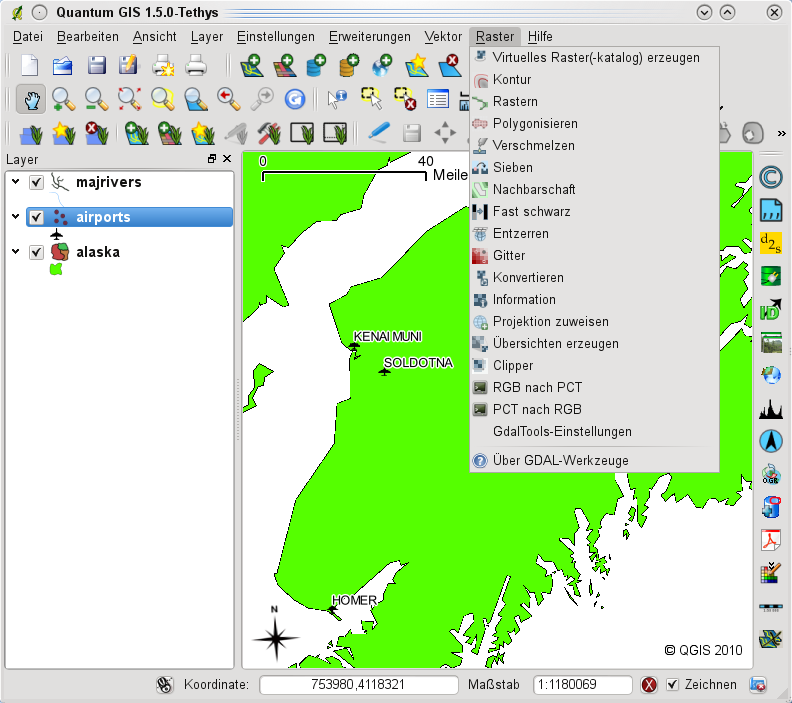
\includegraphics[clip=true, width=12cm]{plugins_gdaltools_images/raster_menu}
\end{figure}

\subsection{Examples}\label{gdal_examples}
Below are some examples of use of the tools.
\subsection{Getting information about a raster}
\begin{figure}[ht]
   \centering
   \caption{\label{gdalinfo}The \emph{Information} dialog window \nixcaption}
   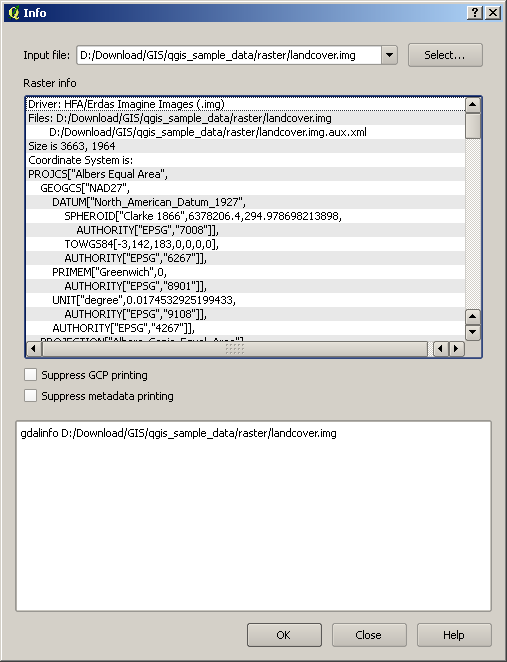
\includegraphics[clip=true, width=12cm]{plugins_gdaltools_images/gdalinfo}
\end{figure}

\minisec{Creating contour lines}
This example will create contour lines from an SRTM elevation tile.
\begin{figure}[ht]
   \centering
   \caption{\label{gdal_contour} The \emph{Contours} dialog window \nixcaption}
   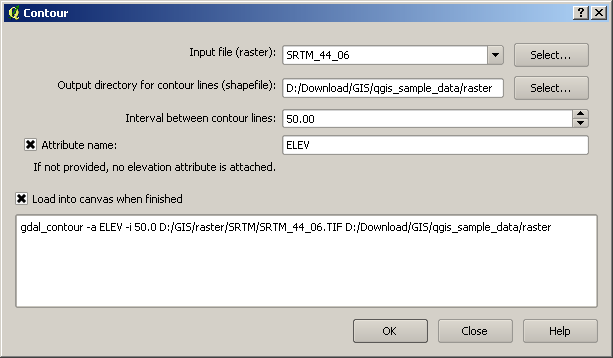
\includegraphics[clip=true, width=12cm]{plugins_gdaltools_images/gdal_contour}
\end{figure}
and the result:
\begin{figure}[ht]
   \centering
   \caption{\label{gdal_contour} The resulting contours layer \nixcaption}
   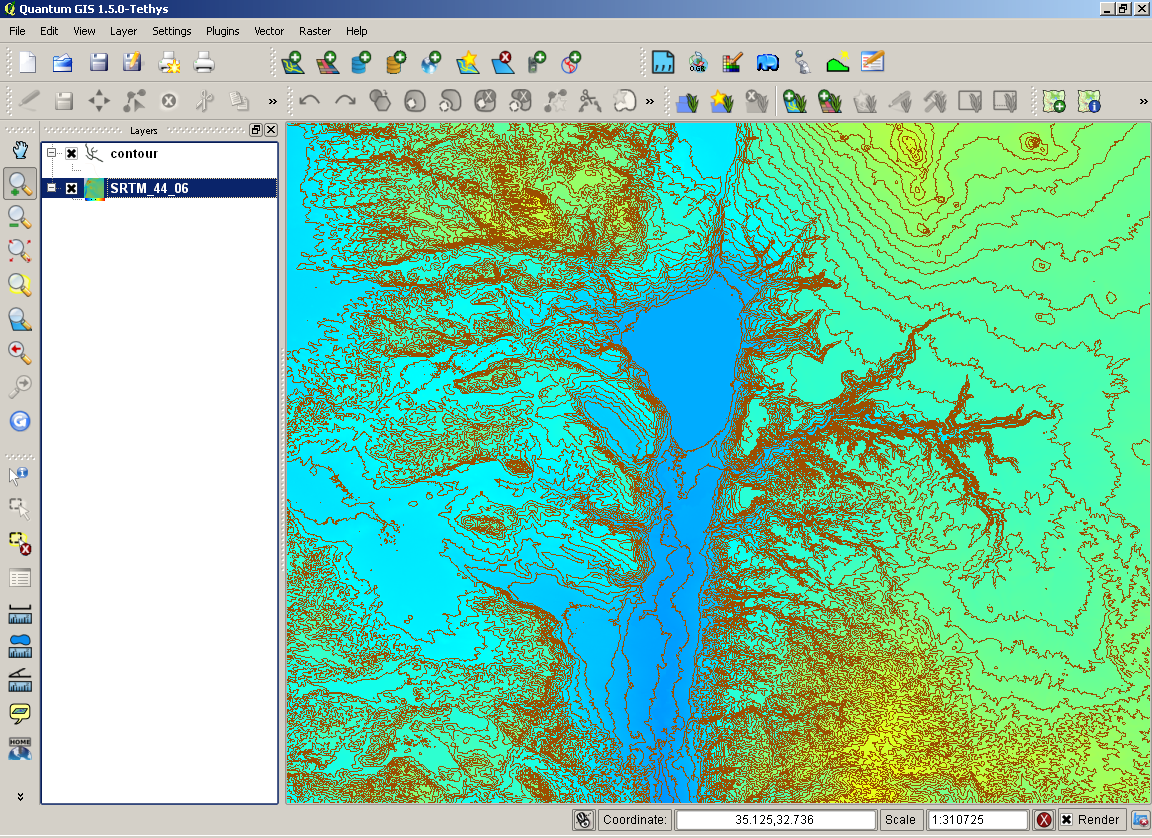
\includegraphics[clip=true, width=12cm]{plugins_gdaltools_images/qgis_contours}
\end{figure}

\minisec{Using GDALwarp to reproject a raster}
Here's the dialog window for reprojecting a landcover image, originally in the Albers Equal Area projection for Alaska (from the QGIS sample dataset) into Lon/Lat WGS84 (EPSG:4326).
\begin{figure}[ht]
   \centering
   \caption{\label{gdalwarp} The \emph{GDAL warp} dialog window \nixcaption}
   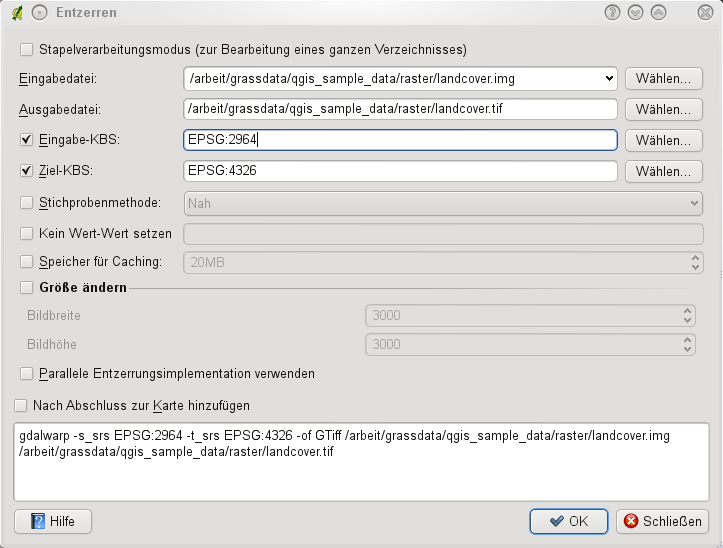
\includegraphics[clip=true, width=12cm]{plugins_gdaltools_images/gdalwarp}
\end{figure}

\FloatBarrier
